\documentclass[11pt,a4paper]{article}
\usepackage{fontspec}
\setmainfont{Times New Roman}
\setsansfont{Segoe UI}
\setmonofont{Consolas}
\usepackage[top=0.42in, bottom=0.42in, left=0.68in, right=0.68in, headheight=0pt, headsep=0pt]{geometry}
\usepackage{amsmath,amssymb}
\usepackage{xcolor}
\usepackage{tikz}
\usetikzlibrary{arrows.meta,positioning,calc,decorations.pathreplacing}
\usepackage{tcolorbox}
\usepackage{hyperref}
\usepackage{booktabs}
\usepackage{caption}

\hypersetup{
    colorlinks=true,
    linkcolor=blue!70!black,
    citecolor=blue!70!black,
    urlcolor=blue!70!black
}

% Custom Callout Boxes matching math_tools_en / house style
\newtcolorbox{learningobj}{
    colback=blue!3!white,
    colframe=blue!60!black,
    fonttitle=\bfseries\sffamily,
    fontupper=\small,
    title={$\blacktriangleright$ MỤC TIÊU HỌC TẬP},
    arc=1.5mm,
    boxrule=0.8pt,
    left=3mm, right=3mm, top=1.0mm, bottom=1.0mm,
    before skip=0.8mm, after skip=1.2mm
}

\newtcolorbox{groundbreaking}{
    colback=teal!4!white,
    colframe=teal!60!black,
    fonttitle=\bfseries\sffamily,
    fontupper=\small,
    title={$\bigstar$ PHÁT HIỆN THEN CHỐT},
    arc=1.5mm,
    boxrule=0.8pt,
    left=3mm, right=3mm, top=1.0mm, bottom=1.0mm,
    before skip=1.0mm, after skip=0.8mm
}

\newtcolorbox{physicalinsight}{
    colback=yellow!6!white,
    colframe=orange!75!black,
    fonttitle=\bfseries\sffamily,
    fontupper=\small,
    title={$\blacktriangleright$ NHÌN THẤY VẬT LÝ},
    arc=1.5mm,
    boxrule=0.8pt,
    left=3mm, right=3mm, top=1.0mm, bottom=1.0mm,
    before skip=1.5mm, after skip=3.5mm
}

\renewcommand{\thefigure}{1.3\alph{figure}}

\begin{document}

% ============================================================================
% TRANG 1: Sóng Dò & Chiếu Vuông Pha
% ============================================================================
\vspace*{-4.5mm}
\section*{1.3 Mô Hình Hóa Toán Học: STFT và Ngân Hàng Bộ Lọc Mel}
\vspace{-2.5mm}

\begin{learningobj}
Thay vì ghi nhớ sáu công thức DSP rời rạc, mục này suy diễn từng toán tử từ các nguyên lý vật lý gốc: sóng dò nhận diện cộng hưởng họa âm, cửa sổ thuôn triệt tiêu bước nhảy biên, phép biến đổi Fourier thời gian ngắn (STFT) hóa giải sự đánh đổi bất định Gabor-Heisenberg, phổ công suất loại bỏ pha dư thừa, ngân hàng bộ lọc Mel uốn thang Hertz tuyến tính theo sinh học ốc tai, và nén logarit mô phỏng độ to cảm nhận của con người. Mọi công thức đều được giải phẫu nghiêm ngặt theo khung năm nhịp: công thức, ký hiệu, ý nghĩa vật lý, giá phần cứng, và điều công thức giấu.
\end{learningobj}

\vspace{0.5mm}
Mục 1.2 đã xây dựng đường truyền dữ liệu (datapath) đóng gói áp suất không khí dạng dòng thành các khung. Mục 1.3 là chiếc kính hiển vi toán học đặt lên một gói dữ liệu đơn lẻ, suy diễn từng toán tử biến đổi phổ từ hiện tượng giao thoa sóng và cơ chế cảm nhận thính giác.

Sáu biểu thức biến dòng mẫu thành 80 con số: (1)~Khung sau áp cửa sổ, (2)~STFT, (3)~Phổ công suất, (4)~Ánh xạ Mel, (5)~Ngân hàng bộ lọc Mel, và (6)~Nén logarit. Các thông số chuẩn: $f_s = 16.000\text{ Hz}$, chiều dài khung $L = 400$ ($25\text{ ms}$), bước nhảy $H = 160$ ($10\text{ ms}$), kích thước FFT $N = 512$, số bộ lọc $M = 80$, $f_{\min} = 0\text{ Hz}$, $f_{\max} = 8.000\text{ Hz}$.

\vspace{-1.5mm}
\subsection*{Sóng Dò, Trước Công Thức}
\vspace{-2mm}

Làm sao một mạch số biết gói âm thanh $x_\ell[n]$ có dao động ở tần số $f_k$? Trong vật lý cổ điển, hiện tượng cộng hưởng được phát hiện bằng cách thăm dò: một bộ dao động chuẩn nội bộ đánh giá sự giao thoa với tín hiệu đầu vào thông qua tích vô hướng $\int_0^T x(t) \cos(\omega_k t) \, dt$. Nếu $x(t)$ chứa tần số $\omega_k$ cùng pha ($\cos(\omega_k t)$), tích số thành $\cos^2(\omega_k t) = \frac{1 + \cos(2\omega_k t)}{2}$. Tích phân trên $T$, họa âm $2\omega_k$ triệt tiêu về 0, để lại phần tích lũy DC dương bằng $\frac{T}{2}$. Nếu $x(t)$ dao động tại bất kỳ họa âm nào khác $\omega_m$ ($m \ne k$), tích phân bằng đúng 0. Sóng dò chỉ cộng hưởng duy nhất với đúng tần số của nó.

Bây giờ hãy vạch trần tử huyệt của một sóng dò đơn lẻ: \textbf{sự mù pha} (phase blindness). Nếu gói âm thanh đến trễ một phần tư chu kỳ (lệch pha $\pi/2$, biến đầu vào thành $\sin(\omega_k t)$), tích số trở thành $\sin(\omega_k t)\cos(\omega_k t) = \frac{1}{2}\sin(2\omega_k t)$. Tích phân trên khoảng $T$ cho kết quả đúng bằng 0: $\int_0^T \sin(\omega_k t) \cos(\omega_k t) \, dt = 0$. Sóng dò đơn lẻ báo mức năng lượng bằng 0 trong khi một âm thanh thực tế đang dội vang qua bộ chuyển đổi.

Để xóa bỏ sự mù pha, ta phải thẩm tra sóng âm bằng \textbf{hai sóng dò trực giao vuông pha} (quadrature): sóng dò đồng pha $\cos(\omega_k t)$ và sóng dò vuông pha $-\sin(\omega_k t)$ (lệch pha $90^\circ$). Đập vào bộ tách sóng hai nhánh này, hai nhánh đo được $A \cos\theta$ và $A \sin\theta$. Theo định lý Pythagoras, biên độ toàn phần được khôi phục với sự miễn nhiễm pha tuyệt đối: $A = \sqrt{(A\cos\theta)^2 + (A\sin\theta)^2}$. Đồng nhất thức Euler, $e^{-j\theta} = \cos\theta - j\sin\theta$, chính là chiếc vỏ bọc đại số của máy thu vuông pha phần cứng hai kênh này.

\vspace{-3.5mm}
\begin{center}
\begin{minipage}{\textwidth}
\centering
\resizebox{0.94\textwidth}{!}{% Figure 1.3a: Giao thoa kế vuông pha sóng dò (Bản tiếng Việt)
\begin{tikzpicture}[
  >=Stealth,
  font=\small,
  blk/.style={draw=black!75, rounded corners=3pt, fill=blue!8, semithick, align=center, inner sep=3pt},
  mathnode/.style={draw=black!75, circle, fill=yellow!20, thick, inner sep=1pt, minimum size=6.5mm},
  accum/.style={draw=black!75, rounded corners=3pt, fill=teal!12, semithick, align=center, inner sep=3pt},
  outnode/.style={draw=black!85, rounded corners=3pt, fill=green!12, thick, align=center, inner sep=3pt},
  wavebox/.style={draw=black!60, fill=white, thin, inner sep=2pt, align=center},
  arrow/.style={->, thick, black!75}
]

% Khung đầu vào
\node[blk, fill=blue!10, text width=2.4cm] (input) at (1.3, 0) {
  \textbf{Khung đầu vào}\\
  $x_\ell[n]$\\
  \scriptsize $0 \le n < N$ ($N{=}512$)
};

% Điểm rẽ nhánh
\coordinate (split) at (3.0, 0);
\filldraw[black!80] (split) circle (2.2pt);
\draw[arrow] (input) -- (split);

% Tách hai nhánh trực giao
\coordinate (c_in) at (3.0, 0.9);
\coordinate (s_in) at (3.0, -0.9);
\draw[thick, black!75] (split) -- (c_in);
\draw[thick, black!75] (split) -- (s_in);

% Nhánh trên: Cosine (Đồng pha)
\node[mathnode] (mul_cos) at (4.9, 0.9) {\large $\times$};
\draw[arrow] (c_in) -- (mul_cos);

\node[wavebox, text width=2.7cm] (probe_cos) at (4.9, 1.85) {
  \scriptsize\textbf{Đồng pha} $\cos\left(\frac{2\pi k n}{N}\right)$\\[0.3mm]
  \begin{tikzpicture}[scale=0.18]
    \draw[->, gray!60] (0,0) -- (6.0,0);
    \draw[blue!75!black, thick, domain=0:6.28, samples=30] plot (\x, {sin(\x r + 1.57 r)});
  \end{tikzpicture}
};
\draw[arrow, blue!75!black] (probe_cos) -- (mul_cos);

\node[accum, text width=2.5cm] (acc_cos) at (8.1, 0.9) {
  \textbf{Bộ tích lũy}\\
  $\sum_{n=0}^{N-1} (\cdot)$\\[0.5mm]
  \scriptsize Tổng dồn
};
\draw[arrow] (mul_cos) -- (acc_cos);

\node[outnode, text width=2.4cm] (re_out) at (11.3, 0.9) {
  \textbf{Phần thực}\\
  $\text{Re}(X_\ell[k])$\\[0.5mm]
  \scriptsize Điểm đồng pha
};
\draw[arrow] (acc_cos) -- (re_out);

% Nhánh dưới: Sine (Vuông pha)
\node[mathnode] (mul_sin) at (4.9, -0.9) {\large $\times$};
\draw[arrow] (s_in) -- (mul_sin);

\node[wavebox, text width=2.7cm] (probe_sin) at (4.9, -1.85) {
  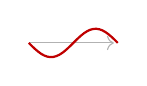
\begin{tikzpicture}[scale=0.18]
    \draw[->, gray!60] (0,0) -- (6.0,0);
    \draw[red!75!black, thick, domain=0:6.28, samples=30] plot (\x, {-sin(\x r)});
  \end{tikzpicture}\\[0.3mm]
  \scriptsize\textbf{Vuông pha} $-\sin\left(\frac{2\pi k n}{N}\right)$
};
\draw[arrow, red!75!black] (probe_sin) -- (mul_sin);

\node[accum, text width=2.5cm] (acc_sin) at (8.1, -0.9) {
  \textbf{Bộ tích lũy}\\
  $\sum_{n=0}^{N-1} (\cdot)$\\[0.5mm]
  \scriptsize Tổng dồn
};
\draw[arrow] (mul_sin) -- (acc_sin);

\node[outnode, text width=2.4cm] (im_out) at (11.3, -0.9) {
  \textbf{Phần ảo}\\
  $\text{Im}(X_\ell[k])$\\[0.5mm]
  \scriptsize Điểm vuông pha
};
\draw[arrow] (acc_sin) -- (im_out);

% Ghép thành bin phổ phức
\node[draw=purple!80!black, rounded corners=4pt, fill=purple!8, thick, align=center, text width=3.4cm] (euler) at (14.8, 0) {
  \textbf{Bin phổ phức}\\[0.8mm]
  $X_\ell[k] = \text{Re} + j\,\text{Im}$\\[1mm]
  \scriptsize \textbf{Vỏ bọc Euler:}\\[0.3mm]
  $\sum_{n=0}^{N-1} x_\ell[n]\, e^{-j\frac{2\pi kn}{N}}$
};

\draw[arrow, purple!80!black] (re_out.east) -- ++(0.3, 0) |- (euler.north west);
\draw[arrow, purple!80!black] (im_out.east) -- ++(0.3, 0) |- (euler.south west);

\end{tikzpicture}
}\\[0.5mm]
\begin{minipage}{0.96\textwidth}
\small\textbf{Hình 1.3a}: \textbf{Giao thoa kế vuông pha sóng dò.} (1)~\textbf{Bản chất:} Kiến trúc bên trong của một bin tần số Fourier được đánh giá như một máy thu tương quan hai nhánh. (2)~\textbf{Điểm cần quan sát:} Khung đầu vào $x_\ell[n]$ tách thành hai nhánh nhân với $\cos(2\pi kn/N)$ (đồng pha) và $-\sin(2\pi kn/N)$ (vuông pha), tích lũy thành tọa độ thực và ảo. (3)~\textbf{Ý nghĩa:} Số phức chính là hai trục trực giao cần thiết để đo năng lượng sóng độc lập với pha xuất hiện.
\end{minipage}
\end{minipage}
\end{center}
\vspace{-3.5mm}

\begin{groundbreaking}
Một bin phổ phức là một máy thu vuông pha phần cứng hai kênh: hai bộ dao động chuẩn trực giao ($\cos$ và $-\!\sin$) đập nhịp cùng sóng áp suất đầu vào, trả về hai điểm số tương đồng giúp khôi phục biên độ tín hiệu bất biến trước pha xuất hiện.
\end{groundbreaking}

\clearpage

% ============================================================================
% TRANG 2: Toán tử 1 (Khung Sau Áp Cửa Sổ) & Hình 6
% ============================================================================
\vspace*{-4.5mm}
\subsection*{1. Khung Sau Áp Cửa Sổ}
\vspace{-2mm}

Để triệt tiêu các bước nhảy biên nhân tạo tại ranh giới khung, gói âm thanh thô được thuôn mượt dần về 0 trước khi giải tích phổ.

\subsubsection*{Giải Phẫu 5 Nhịp: Khung Sau Áp Cửa Sổ}
\vspace{-2mm}
{\small
\textbf{Nhịp 1: Công Thức.} $x_\ell[n] = x[n_0 + \ell H + n] \, w[n], \quad n = 0, 1, \dots, L-1$; tiếp nối bởi bước đệm thêm số 0: $x_\ell[n] = 0, \quad L \le n < N$.\\[1mm]
\textbf{Nhịp 2: Ký Hiệu.} $x_\ell[n]$ là khung sau áp cửa sổ $\ell$ ($L = 400$ mẫu, $25\text{ ms}$ ở $f_s = 16.000\text{ Hz}$); $x$ là dòng âm thanh liên tục; $H = 160$ mẫu ($10\text{ ms}$); $L = 400$ mẫu ($25\text{ ms}$); $w[n]$ là cửa sổ đối xứng Hamming, thuôn dần hai mép ranh giới về $w[0] = w[L-1] = 0{,}08$ và đạt đỉnh $1{,}00$ ở chính giữa.\\[1mm]
\textbf{Nhịp 3: Ý Nghĩa Vật Lý.} Cắt phẳng tín hiệu bằng nhát cắt chữ nhật tương đương với nhân với hàm chữ nhật, cuộn phổ gốc với hàm sinc có các búp phụ suy hao chậm (búp phụ đầu tiên nhô cao $-13\text{ dB}$). Cửa sổ Hamming thuôn hai mép về $0{,}08$, nén búp phụ đầu tiên xuống $-44\text{ dB}$---giảm rò rỉ phổ giả mạo tới $31\text{ dB}$.
}

\vspace{-3mm}
\begin{center}
\begin{minipage}{\textwidth}
\centering
\resizebox{0.94\textwidth}{!}{%
\begin{tikzpicture}[>=Stealth, font=\small]
  % Grid and Axes
  \draw[->, black!75, thick] (-6.8, -5.0) -- (6.8, -5.0) node[right, font=\scriptsize\bfseries] {Độ lệch tần số so với tâm (Hz)};
  \draw[->, black!75, thick] (0, -5.2) -- (0, 0.6) node[above, font=\scriptsize\bfseries] {Độ suy giảm chuẩn hóa (dB)};

  % Horizontal grid lines and dB tick labels
  \foreach \y/\lbl in {0/{0}, -1.3/{-13}, -2.6/{-26}, -4.4/{-44}} {
    \draw[gray!30, thin] (-6.5, \y) -- (6.5, \y);
    \node[left, font=\scriptsize, text=gray!80] at (-6.5, \y) {\lbl~dB};
  }
  % Vertical grid lines and Hz tick labels
  \foreach \x/\lbl in {-4.8/{-160}, -2.4/{-80}, 0/{0}, 2.4/{80}, 4.8/{160}} {
    \draw[gray!30, thin] (\x, -5.0) -- (\x, 0.4);
    \node[below, font=\scriptsize, text=gray!80] at (\x, -5.0) {\lbl};
  }

  % Rectangular window spectrum (sinc shape, blue dashed)
  \draw[blue!80!black, thick, dashed] 
    (-6.5, -2.6) -- (-6.0, -2.5) -- (-5.4, -4.8) -- (-4.8, -2.2) -- (-4.2, -4.8) 
    -- (-3.6, -1.9) -- (-3.0, -4.8) -- (-2.4, -1.6) -- (-1.8, -1.3) -- (-1.2, -4.8) 
    -- (0, 0) 
    -- (1.2, -4.8) -- (1.8, -1.3) -- (2.4, -1.6) -- (3.0, -4.8) -- (3.6, -1.9) 
    -- (4.2, -4.8) -- (4.8, -2.2) -- (5.4, -4.8) -- (6.0, -2.5) -- (6.5, -2.6);

  % Hamming window spectrum (broader main lobe, heavily suppressed side lobes, red solid)
  \draw[red!80!black, ultra thick] 
    (-6.5, -4.5) -- (-5.5, -4.4) -- (-4.5, -4.5) -- (-3.5, -4.4) -- (-2.4, -4.4) 
    -- (-1.6, -2.2) -- (0, 0) -- (1.6, -2.2) -- (2.4, -4.4) 
    -- (3.5, -4.4) -- (4.5, -4.5) -- (5.5, -4.4) -- (6.5, -4.5);

  % Annotations: Both Callout Boxes placed fully inside with generous margins (no clipping)
  \node[draw=blue!80!black, fill=blue!5, rounded corners=3pt, font=\footnotesize, align=left] (rect_box) at (-3.9, -0.9) {
    \textbf{Cửa sổ chữ nhật:}\\[0.5mm]
    Búp chính: $\Delta f = 80\text{ Hz}$ ($2f_s/L$)\\[0.5mm]
    Búp phụ đầu: $\mathbf{-13\text{ dB}}$
  };
  \draw[->, blue!80!black, semithick] (rect_box.east) -- (-1.9, -1.3);

  \node[draw=red!80!black, fill=red!5, rounded corners=3pt, font=\footnotesize, align=left] (hamm_box) at (3.9, -0.9) {
    \textbf{Cửa sổ Hamming:}\\[0.5mm]
    Búp chính: $\Delta f = 160\text{ Hz}$ ($4f_s/L$)\\[0.5mm]
    Búp phụ đầu: $\mathbf{-44\text{ dB}}$
  };
  \draw[->, red!80!black, semithick] (hamm_box.south) -- (3.9, -4.3);

  % Suppression Arrow
  \draw[<->, purple!85!black, very thick] (1.8, -1.3) -- (1.8, -4.4) 
    node[midway, right, font=\footnotesize\bfseries] {Triệt tiêu $+31\text{ dB}$};
\end{tikzpicture}%
}\\[1mm]
\begin{minipage}{0.96\textwidth}
\small\textbf{Hình 6}: \textbf{Rò rỉ phổ: Cửa sổ chữ nhật so với cửa sổ Hamming ($L = 400$, $f_s = 16\text{ kHz}$).} (1)~\textbf{Bản chất:} Hàm truyền đạt phổ khi áp cửa sổ chữ nhật so với Hamming. (2)~\textbf{Điểm cần quan sát:} Búp chính tăng gấp đôi độ rộng ($80\text{ Hz} \to 160\text{ Hz}$), nhưng búp phụ đầu tiên rơi từ $-13\text{ dB}$ xuống $-44\text{ dB}$ (triệt tiêu thêm $31\text{ dB}$). (3)~\textbf{Ý nghĩa:} Áp cửa sổ đánh đổi độ sắc nét tần số lấy dải động, ngăn các formant âm lượng lớn che lấp họa âm phụ âm nhỏ.
\end{minipage}
\end{minipage}
\end{center}
\vspace{-3.5mm}

\begin{physicalinsight}
Áp cửa sổ là một thỏa hiệp bắt buộc với nguyên lý bất định: ta chấp nhận tăng gấp đôi độ rộng búp chính (từ $80\text{ Hz}$ lên $160\text{ Hz}$) để đổi lấy $31\text{ dB}$ triệt tiêu búp phụ. Nếu không triệt tiêu rò rỉ phổ, năng lượng khổng lồ từ các họa âm cơ bản trầm sẽ làm lu mờ hoàn toàn các formant cao tần tinh tế trên toàn phổ.
\end{physicalinsight}

\vspace{1mm}
{\small
\textbf{Nhịp 4: Giá Phần Cứng.} Tiêu tốn $L = 400$ phép nhân số thực trên mỗi khung $10\text{ ms}$. Các hệ số cửa sổ đối xứng được lưu sẵn trong bảng tra trên chip. Các bộ nhân tạo đường ống hoàn tất tầng này dễ dàng trong nhịp khung. Số lát cắt phần cứng chính xác được phân tích ở Mục 1.4 / Chương 6.\\[1mm]
\textbf{Nhịp 5: Điều Công Thức Giấu.} Cửa sổ thuôn triệt tiêu năng lượng âm học ở hai đầu mút khung, ép các mẫu biên về gần 0. Để không tạo ra điểm mù khiến các biến cố âm học tức thời biến mất không dấu vết, các khung kế tiếp bắt buộc phải gối đầu sâu: bước nhảy $H = 160$ mẫu chỉ tiến thêm $40\%$ chiều dài cửa sổ, để lại vùng gối đầu $60\%$ ($L - H = 240$ mẫu chia sẻ) bảo đảm năng lượng âm thanh được bao phủ liên tục, đồng đều dọc theo trục thời gian.
}

\clearpage

% ============================================================================
% TRANG 3: Toán tử 2 (STFT), Toán tử 3 (Phổ Công Suất), Toán tử 4 (Ánh Xạ Mel)
% ============================================================================
\vspace*{-4.5mm}
\subsection*{2. Biến Đổi Fourier Thời Gian Ngắn (STFT)}
\vspace{-2.5mm}
{\small
\textbf{Nhịp 1: Công Thức.} $X_\ell[k] = \sum_{n=0}^{N-1} x_\ell[n] \, e^{-j \frac{2\pi k n}{N}}, \quad k = 0, 1, \dots, N-1$.\\[0.8mm]
\textbf{Nhịp 2: Ký Hiệu.} $k \in \{0, \dots, N-1\}$ là chỉ số bin tần số rời rạc ($f_k = k \frac{f_s}{N} = k \times \frac{16.000}{512} = k \times 31{,}25\text{ Hz}$); $n \in \{0, \dots, N-1\}$ là chỉ số mẫu thời gian; $x_\ell[n]$ được đệm thêm $N - L = 112$ số 0 lên chiều dài $N = 512$; $X_\ell[k]$ là hệ số phổ phức. Nhờ tính đối xứng liên hợp ($X_\ell[N-k] = X_\ell^*[k]$), chỉ cần giữ lại $N/2 + 1 = 257$ bin đầu tiên ($0\text{--}8.000\text{ Hz}$) là bảo toàn trọn vẹn phổ tín hiệu.\\[0.8mm]
\textbf{Nhịp 3: Ý Nghĩa Vật Lý.} Chiếu tín hiệu thời gian 1D sang không gian tọa độ thời gian - tần số phức 2D, cân bằng sự đánh đổi cốt lõi giữa định vị thời gian và độ phân giải tần số (các lát cắt $25\text{ ms}$ tại độ chi tiết $\Delta f = 31{,}25\text{ Hz}$).\\[0.8mm]
\textbf{Nhịp 4: Giá Phần Cứng.} Tính toán trực tiếp tiêu tốn $N$ bin $\times N$ phép nhân - cộng phức mỗi khung $10\text{ ms}$. Thuật toán FFT cơ số 2 giúp người thiết kế không bị kẹt ở $N^2$, giảm khối lượng số học xuống $\frac{N}{2} \log_2 N$ bướm tính toán mỗi khung. Số lát cắt phần cứng chính xác được phân tích ở Mục 1.4 / Chương 6.\\[0.8mm]
\textbf{Nhịp 5: Điều Công Thức Giấu.} Mặc định tín hiệu lặp lại tuần hoàn với chu kỳ $N$. Việc đệm thêm 112 số 0 lên 512 điểm chỉ làm lưới nội suy phổ dày hơn mà không cải thiện độ phân giải tần số vật lý vốn bị chặn bởi chiều dài cửa sổ $L$.
}

\vspace{1.5mm}
\hrule
\vspace{1.5mm}

\subsection*{3. Phổ Công Suất}
\vspace{-2.5mm}
{\small
\textbf{Nhịp 1: Công Thức.} $P_\ell[k] = |X_\ell[k]|^2 = \text{Re}(X_\ell[k])^2 + \text{Im}(X_\ell[k])^2, \quad k = 0, 1, \dots, \frac{N}{2}$.\\[0.8mm]
\textbf{Nhịp 2: Ký Hiệu.} $P_\ell[k] \in \mathbb{R}_{\ge 0}$ là mật độ phổ công suất trên $257$ bin tần số; $\text{Re}(X_\ell[k]), \text{Im}(X_\ell[k])$ là điểm số chiếu đồng pha và vuông pha thu từ STFT.\\[0.8mm]
\textbf{Nhịp 3: Ý Nghĩa Vật Lý.} Nhận dạng giọng nói dựa trên sự phân bố năng lượng formant thay vì góc pha âm học. Bình phương độ lớn loại bỏ góc pha, trích xuất $257$ giá trị năng lượng thực không âm phản ánh cấu trúc ngữ âm.\\[0.8mm]
\textbf{Nhịp 4: Giá Phần Cứng.} Tiêu tốn 2 phép bình phương và 1 phép cộng cho mỗi bin trên $257$ bin mỗi khung $10\text{ ms}$. Tính công suất ($|X|^2$) giúp triệt tiêu hoàn toàn khối tính căn bậc hai phần cứng đắt đỏ. Số lát cắt phần cứng chính xác được phân tích ở Mục 1.4 / Chương 6.\\[0.8mm]
\textbf{Nhịp 5: Điều Công Thức Giấu.} Bỏ pha là biến đổi một chiều không thể đảo ngược. Việc khôi phục lại dạng sóng âm thanh miền thời gian là bất khả thi nếu không có thuật toán ước lượng pha.
}

\vspace{1.5mm}
\hrule
\vspace{1.5mm}

\subsection*{4. Ánh Xạ Tần Số Mel}
\vspace{-2.5mm}
{\small
\textbf{Nhịp 1: Công Thức.} $\mathrm{mel}(f) = 2595 \log_{10}\!\left(1 + \frac{f}{700}\right)$.\\[0.8mm]
\textbf{Nhịp 2: Ký Hiệu.} $f$ là tần số liên tục tính bằng Hertz ($0 \le f \le 8.000\text{ Hz}$); $\mathrm{mel}(f)$ là cao độ cảm nhận tính bằng Mel.\\[0.8mm]
\textbf{Nhịp 3: Ý Nghĩa Vật Lý.} Mô phỏng cơ chế phi tuyến của ốc tai người: nhạy bén ở tần số thấp, thô ráp dần ở tần số cao. Mỗi bước bằng nhau $355\text{ mel}$ (tương ứng $1/8$ toàn dải $2.840\text{ mel}$) chỉ trải $259\text{ Hz}$ ở dải thấp ($0\text{--}259\text{ Hz}$ qua nghịch đảo $700 \times (10^{355/2595} - 1)$), nhưng dãn rộng tới $2.351\text{ Hz}$ ở dải cao nhất ($5.649\text{--}8.000\text{ Hz}$ với $\Delta f = 8.000 - 5.649\text{ Hz}$)---dãn nở tới chín lần về băng thông vật lý.\\[0.8mm]
\textbf{Nhịp 4: Giá Phần Cứng.} Không tiêu tốn logic thời gian chạy. Hàm uốn Mel được tính toán ngoại tuyến khi thiết kế để sinh tần số tâm lưu trong bộ nhớ trên chip.\\[0.8mm]
\textbf{Nhịp 5: Điều Công Thức Giấu.} Đường cong liên tục phải ánh xạ lên lưới bin rời rạc. Ở tần số thấp, bề rộng bộ lọc có thể hẹp hơn khoảng cách bin $\Delta f = 31{,}25\text{ Hz}$ ($16000/512$), gây nguy cơ sai lệch rời rạc hóa.
}

\clearpage

% ============================================================================
% TRANG 4: Toán tử 5 (Ngân Hàng Bộ Lọc Mel Là Tổng Có Trọng Số) + Hình 1.3b
% ============================================================================
\vspace*{-4.5mm}
\subsection*{5. Ngân Hàng Bộ Lọc Mel Là Tổng Có Trọng Số}
\vspace{-2mm}

Để nén các bin tuyến tính thành các kênh cảm nhận, các bộ lọc tam giác tích phân năng lượng qua các dải không đồng đều.

\subsubsection*{Giải Phẫu 5 Nhịp: Ngân Hàng Bộ Lọc Mel}
\vspace{-2mm}
{\small
\textbf{Nhịp 1: Công Thức.} $E_\ell[m] = \sum_{k=0}^{256} g_m[k] \, P_\ell[k], \quad m = 0, 1, \dots, M-1$, với $g_m[k]$ là các hàm trọng số hình tam giác gối chồng:
$g_m[k] = \frac{k - k_{m-1}}{k_m - k_{m-1}}$ khi $k_{m-1} \le k \le k_m$; $g_m[k] = \frac{k_{m+1} - k}{k_{m+1} - k_m}$ khi $k_m < k \le k_{m+1}$; và $0$ ở các vị trí khác.\\[1mm]
\textbf{Nhịp 2: Ký Hiệu.} $m \in \{0, 1, \dots, M-1\}$ là chỉ số dải Mel ($M = 80$); $k_m$ là chỉ số bin FFT của tần số tâm bộ lọc $m$; $g_m[k]$ là trọng số tam giác cho bin $k$ trong bộ lọc $m$; $E_\ell[m]$ là vector năng lượng phổ Mel (kích thước $[1, 80]$).\\[1mm]
\textbf{Nhịp 3: Ý Nghĩa Vật Lý.} 80 bộ lọc tam giác nén 257 bin công suất tuyến tính thành 80 kênh cảm nhận. Từng bộ lọc tích phân năng lượng trong dải, bảo toàn chi tiết phổ tinh vi ở dải nguyên âm tần thấp trong khi gom các dải năng lượng rộng ở dải phụ âm ồn tần cao.
}

\vspace{-3mm}
\begin{center}
\begin{minipage}{\textwidth}
\centering
\resizebox{0.94\textwidth}{!}{% Figure 1.3b: 257 bin FFT tuyến tính ánh xạ vào 80 bộ lọc tam giác Mel (Đo từ bin_points của Lab 1.3)
\begin{tikzpicture}[
  >=Stealth,
  font=\small,
  tri/.style={draw=teal!85!black, thick, fill=teal!12},
  colltri/.style={draw=red!85!black, ultra thick, fill=red!15},
  midtri/.style={draw=blue!85!black, thick, fill=blue!12},
  hightri/.style={draw=purple!85!black, thick, fill=purple!12},
  bin/.style={draw=black!35, thin},
  ax/.style={->, black!75, thick},
  tk/.style={font=\scriptsize, text=black!75},
  ann/.style={font=\footnotesize, text=black!85}
]

% ==================== (a) Toàn bộ dải phổ 0 - 8 kHz ====================
\begin{scope}[x=0.00195cm, y=1.2cm]
  \node[font=\bfseries\small, anchor=west] at (-120, 2.25) 
    {(a) Phân bổ 80 bộ lọc Mel thực tế sinh từ 82 cạnh \texttt{bin\_points} ($\Delta\text{mel} = 35{,}062$, $\text{mel}(8000) = 2840{,}02$)};

  % Trục tần số
  \draw[ax] (-80, 0) -- (8300, 0) node[right, font=\scriptsize\bfseries] {Tần số (Hz)};
  
  \foreach \f in {0, 1000, 2000, 3000, 4000, 5000, 6000, 7000, 8000} {
    \draw[black!60, semithick] (\f, -0.06) -- (\f, 0.06);
  }
  \node[tk, below] at (0, -0.06) {$0$};
  \node[tk, below] at (1000, -0.06) {$1\text{k}$};
  \node[tk, below] at (2000, -0.06) {$2\text{k}$};
  \node[tk, below] at (3000, -0.06) {$3\text{k}$};
  \node[tk, below] at (4000, -0.06) {$4\text{k}$};
  \node[tk, below] at (5000, -0.06) {$5\text{k}$};
  \node[tk, below] at (6000, -0.06) {$6\text{k}$};
  \node[tk, below] at (7000, -0.06) {$7\text{k}$};
  \node[tk, below] at (8000, -0.06) {$8\text{k}$};

  % Các bin FFT tuyến tính bên dưới (tổng cộng 257 bin)
  \fill[black!5] (0, 0) rectangle (8000, 0.08);
  \foreach \b in {0, 32, 64, 96, 128, 160, 192, 224, 256} {
    \pgfmathsetmacro{\hz}{\b * 31.25}
    \draw[bin] (\hz, 0) -- (\hz, 0.70);
    \node[font=\tiny, text=gray!70, anchor=south] at (\hz, 0.70) {$k{=}\b$};
  }

  % Các bộ lọc tam giác thực tế
  % Dải tần thấp (bị sụp mép và hẹp)
  \draw[colltri] (0, 0) -- (0, 0.45) -- (31.25, 0) -- cycle; % Bộ lọc 0 sụp
  \draw[tri] (0, 0) -- (31.25, 0.45) -- (62.5, 0) -- cycle; % Bộ lọc 1
  \draw[colltri] (31.25, 0) -- (62.5, 0.45) -- (62.5, 0) -- cycle; % Bộ lọc 2 sụp

  % Bộ lọc quanh 440 Hz
  \draw[midtri, draw=blue!85!black, fill=blue!15, thick] (406.25, 0) -- (437.5, 0.45) -- (468.75, 0) -- cycle; % Bộ lọc 15 (bin 13, 14, 15)

  % Dải tần trung
  \draw[tri] (980, 0) -- (1135, 0.45) -- (1300, 0) -- cycle;
  \draw[tri] (1850, 0) -- (2080, 0.45) -- (2320, 0) -- cycle;
  \draw[tri] (3200, 0) -- (3550, 0.45) -- (3920, 0) -- cycle;

  % Dải tần cao (rộng, dãn nở)
  \draw[hightri] (5400, 0) -- (5880, 0.45) -- (6390, 0) -- cycle;
  \draw[hightri] (6390, 0) -- (6920, 0.45) -- (7475, 0) -- cycle;
  \draw[hightri] (7475.2, 0) -- (7733.5, 0.45) -- (8000.0, 0) -- cycle; % Bộ lọc 79

  % Chú thích
  \node[ann, align=left, text=red!90!black, anchor=west] at (350, 1.7) {
    \textbf{Tần số thấp:}\\
    Bộ lọc siêu hẹp ($\Delta f \le 31{,}25\text{ Hz}$)\\
    \textbf{3 bộ lọc bị sụp đổ} ($m{=}0, 2, 3$)
  };

  \node[ann, align=right, text=purple!90!black, anchor=east] at (7800, 1.7) {
    \textbf{Bộ lọc $m{=}79$ ($7475\text{--}8000\text{ Hz}$):}\\
    Phủ bin 239 đến bin 256 ($17\text{ bin}$)\\
    Dãn rộng $\Delta f \approx 525\text{ Hz}$
  };
\end{scope}

% ==================== (b) So sánh vi mô: Sự sụp đổ vs Dãn nở ====================
\begin{scope}[yshift=-3.1cm, y=1.0cm]
  \node[font=\bfseries\small, anchor=west] at (-0.3, 2.1) 
    {(b) Hiện thực chi tiết từng bin: Bộ lọc 0 sụp đổ, Bộ lọc 15 bắt đỉnh 440 Hz, Bộ lọc 79 dãn nở};

  % Hộp 1: Bộ lọc 0 sụp đổ (bên trái)
  \draw[draw=gray!50, fill=gray!4, rounded corners=3pt] (-0.3, -0.9) rectangle (4.9, 1.8);
  \node[font=\scriptsize\bfseries, text=red!85!black, anchor=north west] at (-0.2, 1.7) 
    {Bộ lọc $m{=}0$ (sụp trái): $[0, 0, 1]$};

  \foreach \i/\freq in {0/0, 1/31.25, 2/62.5} {
    \pgfmathsetmacro{\bx}{0.2 + \i * 1.5}
    \draw[fill=blue!10, draw=blue!60] (\bx, -0.55) rectangle ++(1.1, 0.45);
    \node[font=\tiny] at (\bx + 0.55, -0.32) {bin \i};
    \node[font=\tiny, text=gray!70, below] at (\bx + 0.55, -0.55) {\freq};
  }
  % Vẽ tam giác sụp đổ của Bộ lọc 0 (cạnh trái trùng đỉnh tại x=0)
  \draw[colltri] (0.2, 0) -- (0.2, 0.6) -- (1.7, 0) -- cycle;
  \node[font=\scriptsize\bfseries, text=red!85!black] at (0.9, 0.85) {Sụp trái};

  % Hộp 2: Bộ lọc 15 (ở giữa) - ôm đỉnh 440 Hz tại bin 14
  \draw[draw=gray!50, fill=gray!4, rounded corners=3pt] (5.2, -0.9) rectangle (10.4, 1.8);
  \node[font=\scriptsize\bfseries, text=blue!85!black, anchor=north west] at (5.3, 1.7) 
    {Bộ lọc $m{=}15$ (bắt $440\text{ Hz}$): $[13, 14, 15]$};

  \foreach \i/\k/\freq in {0/13/406.2, 1/14/437.5, 2/15/468.8} {
    \pgfmathsetmacro{\bx}{5.6 + \i * 1.5}
    \draw[fill=blue!10, draw=blue!60] (\bx, -0.55) rectangle ++(1.1, 0.45);
    \node[font=\tiny\bfseries] at (\bx + 0.55, -0.32) {bin \k};
    \node[font=\tiny, text=gray!70, below] at (\bx + 0.55, -0.55) {\freq};
  }
  \draw[midtri, ultra thick] (5.6, 0) -- (7.1 + 0.55, 0.6) -- (8.6 + 1.1, 0) -- cycle;
  \node[font=\scriptsize\bfseries, text=blue!85!black] at (7.65, 0.85) {$g_{15}[14] = 1{,}00$};

  % Hộp 3: Bộ lọc 79 (bên phải) - phủ 17 bin
  \draw[draw=gray!50, fill=gray!4, rounded corners=3pt] (10.7, -0.9) rectangle (16.7, 1.8);
  \node[font=\scriptsize\bfseries, text=purple!85!black, anchor=north west] at (10.8, 1.7) 
    {Bộ lọc $m{=}79$ ($7475\text{--}8000\text{ Hz}$): $[239, 247, 256]$};

  \draw[fill=blue!10, draw=blue!60] (11.1, -0.55) rectangle ++(1.2, 0.45) node[midway, font=\tiny] {bin 239};
  \node[font=\tiny, text=gray!70, below] at (11.7, -0.55) {$7475$};
  \node[font=\small] at (12.8, -0.32) {$\cdots$};
  \draw[fill=blue!20, draw=blue!80] (13.4, -0.55) rectangle ++(1.2, 0.45) node[midway, font=\tiny\bfseries] {bin 247};
  \node[font=\tiny, text=gray!70, below] at (14.0, -0.55) {$7733$};
  \node[font=\small] at (15.1, -0.32) {$\cdots$};
  \draw[fill=blue!10, draw=blue!60] (15.4, -0.55) rectangle ++(1.1, 0.45) node[midway, font=\tiny] {bin 256};
  \node[font=\tiny, text=gray!70, below] at (15.95, -0.55) {$8000$};

  \draw[hightri, ultra thick] (11.1, 0) -- (14.0, 0.6) -- (16.5, 0) -- cycle;
  \node[font=\scriptsize\bfseries, text=purple!85!black] at (14.0, 0.85) {Phủ $17\text{ bin}$};
\end{scope}

\end{tikzpicture}
}\\[0.8mm]
\begin{minipage}{0.96\textwidth}
\small\textbf{Hình 1.3b}: \textbf{257 bin FFT tuyến tính sụp đổ dưới 80 bộ lọc tam giác Mel.} (1)~\textbf{Bản chất:} Ánh xạ 257 bin tần số tuyến tính ($0\text{--}8.000\text{ Hz}$) vào 80 bộ lọc tam giác cảm nhận Mel. (2)~\textbf{Điểm cần quan sát:} Ở vùng (a), các bộ lọc tần thấp dày đặc và hẹp, trong khi các bộ lọc cao dãn rộng theo hàm mũ. Ở vùng (b), Dải $m=0$ chỉ tích hợp vài bin, trong khi Dải $m=79$ gom hàng chục bin ($6.593\text{--}8.000\text{ Hz}$). (3)~\textbf{Ý nghĩa:} Ngân hàng bộ lọc tập trung độ phân giải vào các dải formant ngữ âm đồng thời thu gọn mạnh số chiều đầu vào cho mạng nơ-ron.
\end{minipage}
\end{minipage}
\end{center}
\vspace{-3.5mm}

\begin{physicalinsight}
Ngân hàng bộ lọc Mel là một cỗ máy tập trung thông tin bất đối xứng. Ở dải tần thấp ($0\text{--}1\text{ kHz}$) nơi cư trú của cao độ và formant nguyên âm cốt lõi, mỗi dải chỉ tích hợp một vài bin FFT, bảo tồn chi tiết họa âm tinh vi. Ở dải tần cao ($6\text{--}8\text{ kHz}$) nơi phụ âm xát tạo ra tiếng ồn khuếch tán, mỗi dải gom hàng chục bin, giữ lại đường bao năng lượng tổng thể trong khi gạt bỏ cấu trúc vi mô không cần thiết.
\end{physicalinsight}

\vspace{1mm}
{\small
\textbf{Nhịp 4: Giá Phần Cứng.} Tiêu tốn phép nhân ma trận thưa với vector trên mỗi khung. Vì mỗi bin tuyến tính $k$ chỉ rơi vào tối đa hai bộ lọc tam giác kế cận, ma trận phần lớn là số 0. Phần cứng chỉ tốn các phép nhân - cộng trên các nhịp bin tích cực; số lát cắt phần cứng chính xác được phân tích ở Mục 1.4 / Chương 6.\\[1mm]
\textbf{Nhịp 5: Điều Công Thức Giấu.} Bẫy rời rạc hóa: Khi tần số tâm liên tục được làm tròn về chỉ số bin nguyên, các bộ lọc tần thấp kế cận có thể bị sụp về cùng một bin nếu khoảng cách hẹp hơn $\Delta f = 31{,}25\text{ Hz}$ ($16000/512$). Bộ lọc có đỉnh và hai mép trùng nhau sẽ có độ rộng bằng 0 và cho ra năng lượng chết. Phần cứng phải bảo đảm mỗi dải phủ ít nhất một bin duy nhất.
}

\clearpage

% ============================================================================
% TRANG 5: Toán tử 6 (Nén Logarit) & Cầu Nối Sang Mục 1.4
% ============================================================================
\vspace*{-4.5mm}
\subsection*{6. Nén Logarit}
\vspace{-2mm}

Phép biến đổi cuối cùng nén các biến thiên năng lượng vật lý rộng lớn vào một không gian đặc trưng chuẩn hóa, phù hợp cho các tầng mạng nơ-ron.

\subsubsection*{Giải Phẫu 5 Nhịp: Nén Logarit}
\vspace{-2mm}
{\small
\textbf{Nhịp 1: Công Thức.} $S_\ell[m] = \ln\bigl(\max(E_\ell[m], 10^{-6})\bigr), \quad m = 0, 1, \dots, M-1$.\\[1mm]
\textbf{Nhịp 2: Ký Hiệu.} $S_\ell[m]$ là vector đặc trưng log-Mel năng lượng (kích thước $[1, 80]$) phát cho mô hình âm học; $E_\ell[m]$ là năng lượng dải Mel thô từ Toán tử 5; $10^{-6}$ là ngưỡng chặn dưới ngăn thảm họa $\ln(0) \to -\infty$ khi gặp khoảng lặng.\\[1mm]
\textbf{Nhịp 3: Ý Nghĩa Vật Lý.} Cảm nhận độ to của con người tỷ lệ logarit với công suất âm thanh. Trong môi trường thực tế, áp suất âm thanh dao động từ tiếng thì thầm khẽ ($10^{-5}\text{ Pa}$) đến tiếng thét lớn ($10\text{ Pa}$)---chênh lệch năng lượng tới $10^{10}$, tương đương $100\text{ dB}$. Nén logarit điều hòa dải động khổng lồ này về một phân phối số học gọn gàng. Hơn nữa, phép logarit biến các hiệu ứng kênh có tính chất nhân (như khoảng cách micro hay âm học phòng) thành các độ lệch cộng tính đơn giản.\\[1mm]
\textbf{Nhịp 4: Giá Phần Cứng.} Tiêu tốn 80 phép tính logarit trên mỗi khung $10\text{ ms}$. Trên phần cứng, logarit được đánh giá bằng bảng tra hoặc xấp xỉ đa thức từng đoạn. Số lát cắt phần cứng chính xác được phân tích ở Mục 1.4 / Chương 6.\\[1mm]
\textbf{Nhịp 5: Điều Công Thức Giấu.} Đạo hàm của logarit tự nhiên, $\frac{d}{dx}\ln(x) = \frac{1}{x}$, phân kỳ về vô hạn khi $x \to 0$. Dù ngưỡng chặn $10^{-6}$ ngăn được âm vô cùng, những dao động nhiễu siêu nhỏ quanh ngưỡng sàn vẫn tạo ra các biến động lớn trong không gian đặc trưng, đòi hỏi xử lý số học cẩn trọng trong quá trình lượng tử hóa dấu phẩy tĩnh.
}

\vspace{5mm}
\hrule
\vspace{5mm}

\subsection*{Thực Tế Silicon: Cầu Nối Sang Mục 1.4}

Các dẫn xuất toán học của STFT và ngân hàng bộ lọc Mel trong mục này giả định số học vô hạn độ chính xác, truy xuất bộ nhớ trễ bằng 0 và thực thi tức thời. Trên máy tính phát triển, những phương trình này chạy mượt mà trong môi trường khoa học Python, nơi bộ nhớ dồi dào và phần cứng dấu phẩy động che giấu hạn chót xử lý $10\text{ ms}$ cùng ngân sách nhiệt.

Khi chuỗi toán học này được đẩy xuống silicon biên vật lý vận hành dưới trần công suất ngặt nghèo ($< 15\text{ W}$) với hạn chót cứng $10\text{ ms}$ cho mỗi khung, các công thức trừu tượng va chạm trực diện với các ràng buộc phần cứng vật lý. Liệu một GPU biên hay một cấu trúc không gian FPGA có thể thỏa mãn các hạn chót âm thanh dạng dòng này hay không chính là câu hỏi kiến trúc được khám phá tiếp theo.

\end{document}
